\documentclass{beamer}
\usetheme{Dresden}
\usepackage[utf8]{inputenc}

\title{Abschlusspräsentation}
\author{Team Ilias}
\date{\today}

\begin{document}
	\maketitle
	\frame{\tableofcontents[]}

	\section{Teamaufteilung}
	\begin{frame}
		\frametitle{Aufteilung des Teams}
		\begin{tabular}{|c|c|}\hline
			Teammitglied & Aufgabe \\\hline
			Josephine Rehak & Chefprogrammiererin\\\hline
			Richard Mörbitz & Assistent\\\hline
			Max Friedrich & Administrator\\\hline
			Peter Merseburger & Testverantwortlicher\\\hline
			Julius Felchow & Sekretär\\\hline
		\end{tabular}
	\end{frame} 
 
	\section{Aufgabe}
		\begin{frame}
			\frametitle{Einführung zur Thematik}
  			Ilias ist eine E-Learning Plattform in der E-					Klausuren erstellt werden können. Ein Fragenpool 				kann erstellt und die Fragen in der Klausur 					genutzt werden.\\
  			\pause
    		Die Reviewmöglichkeit für diese Fragen war unsere 				Aufgabe.
		\end{frame}
		\begin{frame}
			\frametitle{Aufgabenstellung}
			\begin{itemize}
				\item Erstellen einer Reviewbaren Frage
				\item Erstellen von Reviews zu Ilias' Fragen
				\item Händische Zuordnung von Reviewer zu Frage
				\item Übersicht über die eigens erstellten Fragen und Reviews
				
			\end{itemize}
		\end{frame}

		\begin{frame}
			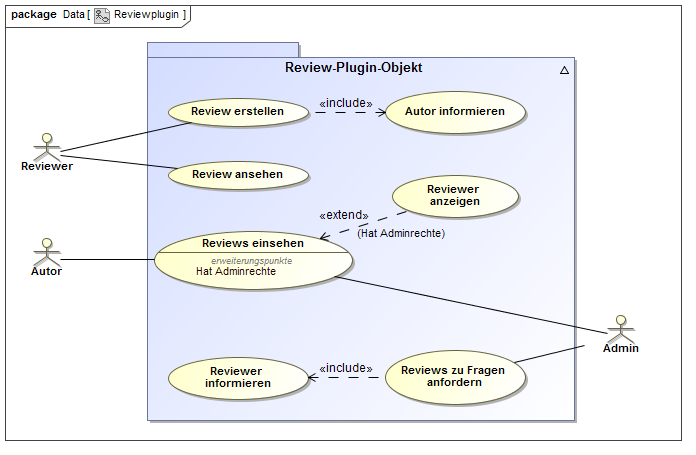
\includegraphics[scale=0.45]{Diagramme/Use_Case_Diagram__Reviewplugin.png}
			\label{Reviewplugin}	
		\end{frame}
		\begin{frame}
			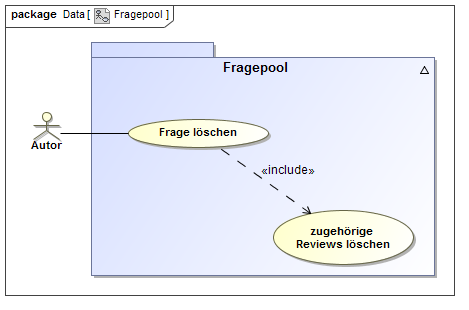
\includegraphics[scale=0.7]{Diagramme/Use_Case_Diagram__Fragepool.png}
				\label{Fragepool}
		\end{frame}
	\section{Probleme}
		\begin{frame}
			\frametitle{Probleme}
    		\begin{itemize}
    			\item Wahl des Repositorys
		    	\item Erstellen der Reviewbaren Fragen
    			\item Wahl der Reviewerzuordnung
    			\item Erstellen der Tests lieferte Probleme
    			\item Import/Export
    			\item Zeitmanagement - Wunschkriterien wurden nicht erfüllt
    		\end{itemize}
		\end{frame}
		\begin{frame}
			Erfüllung der Musskriterien:
			\begin{itemize}
				\item Die Review Maske wurde gemäß Prof. Wollersheims Beispiel-Maske erstellt.
				\item Das angeben der Expertise nach Frau Kombrinks Wunsch ist implementiert.
				\item Die Wissensdimension und Taxonomie des Autors wird angezeigt und der Reviewer muss seine eigene Einschätzung angeben.
				\item "Ghost-Reviewing" wurde implementiert - der Autor erfährt nicht den Namen des Reviewers und andersherum.
				\item Ein Reviewbarer Fragetyp wurde implementiert.	
				\item Die eingegebenen Daten des Reviewers werden gespeichert und stehen dem Autor zum Einsehen zur Verfügung.
				\item Der Administrator hat Zugriff auf die Namen der Autoren und Reviewer.
			\end{itemize}
		\end{frame}

	\section{Vorstellung des Resultats}
		\begin{frame}
		\frametitle{Live-Demo}
		\end{frame}
\end{document}